

\documentclass[9pt]{beamer}

\usepackage[Rbeamer]{Rosenberg}

%\usepackage{Sweave}



\definecolor{ricolor}{rgb}{0.101, 0.043, 0.432}
\newcommand{\ri}[1]{\textcolor{blue}{\tt\smaller #1}}


\title{Common questions (and answers) about \R  }
\author{David M. Rosenberg}
\institute[University of Chicago] % (optional, but mostly needed)
{
  Committee on Neurobiology\\
  University of Chicago
}
% - Use the \inst command only if there are several affiliations.
% - Keep it simple, no one is interested in your street address.

\date{\today}

\subject{Talks}
% This is only inserted into the PDF information catalog. Can be left
% out. 



% If you have a file called "university-logo-filename.xxx", where xxx
% is a graphic format that can be processed by latex or pdflatex,
% resp., then you can add a logo as follows:

% \pgfdeclareimage[height=0.5cm]{university-logo}{university-logo-filename}
% \logo{\pgfuseimage{university-logo}}



% Delete this, if you do not want the table of contents to pop up at
% the beginning of each subsection:
%\AtBeginSection[]
\newcommand{\makeOutline}{%
  \begin{frame}<beamer>{Outline}
    \begin{columns}[c]
      \column{0.5\textwidth}
        \tableofcontents[currentsection,currentsubsection]
    \end{columns}
  \end{frame}
}

\AtBeginSection[]
{
  \begin{frame}<beamer>{Outline}
  \begin{columns}[c]
  \column{0.5\textwidth}
    \tableofcontents[currentsection,sections={<1-3>}]
  \column{0.5\textwidth}
    \tableofcontents[currentsection,sections={<4-5>}]
  \end{columns}
  \end{frame}
}


% If you wish to uncover everything in a step-wise fashion, uncomment
% the following command: 

%\beamerdefaultoverlayspecification{<+->}


\begin{document}

\begin{frame}
  \titlepage
\end{frame}

% \begin{frame}<beamer>{Outline}
%   \begin{columns}[c]
%   \column{0.5\textwidth}
%     \tableofcontents[sections={<1-3>}]
%   \column{0.5\textwidth}
%     \tableofcontents[sections={<4-5>}]
%   \end{columns}
% \end{frame}


% Since this a solution template for a generic talk, very little can
% be said about how it should be structured. However, the talk length
% of between 15min and 45min and the theme suggest that you stick to
% the following rules:  

% - Exactly two or three sections (other than the summary).
% - At *most* three subsections per section.
% - Talk about 30s to 2min per frame. So there should be between about
%   15 and 30 frames, all told.

\section{Admin issues}
\subsection{Things to ask for}

\begin{frame}{Admin issues}{Things to ask for}
\begin{itemize}[<+->]
  \item \textbf{Email addresses:}\\
    If you use a non-University of Chicago email account, let me know either via an email from your {\tt uchicago.edu} email account or a written note.
  \end{itemize}
  \begin{onlyenv}<2->\begin{itemize}[<+->]
    \item \textbf{Use of lab time:}\\
      What do you think would be the best use of your time in lab.
      \begin{itemize}[<+->]
        \item Status quo.  Labs are principally time for you to try to work on the lab.
        \item \emph{Short} lectures. Presentations like this (but shorter; 10-20 minutes) at the start / end / middle of labs seems helpful.
        \item Review of the previous week's assignment and / or group discussion of the different ways you solved the problems.
        \item Discussion / question-and-answer time about the topics and concepts presented in lecture \emph{not} directly pertaining to computational programming.
      \end{itemize}
\end{itemize}
\end{onlyenv}
\end{frame}

  

\subsection{Things to provide}

\begin{frame}{Admin issues}{Things to provide}
  \begin{itemize}[<+->]
    \item \textbf{Homework examples \& template:}\\
      Files on chalk.
    \item \textbf{Grades \& comments:}\\
      By next week you will have exercises 0 and 1 returned to you.
    \item \textbf{Tools \& utilities:}\\
      Source code ``cleaner,'' problem uploader
    \item \textbf{Cheat sheets:}\\
      Math ``cheat sheets'' (i.e. trigonometric identities, tables of common integrals and derivatives, etc.) as well as ``cheat sheets'' for \R are in progress.
  \end{itemize}
\end{frame}    



\section{Manipulating Data - Vectors}

\subsection{Basic usage}

\begin{frame}[fragile]{Manipulating Data - Vectors}{Basic usage}
  \begin{columns}
    \column{0.5\textwidth}
  \begin{itemize}
    \item Rules \medskip
    \begin{itemize}
      \item Single type \smallskip
      \item Accessed by index \smallskip
      \item Can be named or unnamed \smallskip
    \end{itemize}
  \end{itemize}
\begin{Schunk}
\begin{Sinput}
>c('hello', TRUE); c(1, TRUE)
\end{Sinput}
\begin{Soutput}
[1] "hello" "TRUE" 
\end{Soutput}
\begin{Soutput}
[1] 1 1
\end{Soutput}
\begin{Sinput}
>class(c('hello', TRUE)); class(c(1, TRUE));
\end{Sinput}
\begin{Soutput}
[1] "character"
\end{Soutput}
\begin{Soutput}
[1] "numeric"
\end{Soutput}
\begin{Sinput}
>c('Hello', 14);
\end{Sinput}
\begin{Soutput}
[1] "Hello" "14"   
\end{Soutput}
\begin{Sinput}
>class(c(TRUE, TRUE));
\end{Sinput}
\begin{Soutput}
[1] "logical"
\end{Soutput}
\end{Schunk}
    \column{0.5\textwidth}
\begin{Schunk}
\begin{Sinput}
>my_name <- c('D', 'a', 'v', 'i',
              'd', ' ', 'R', '.');
>length(my_name);
\end{Sinput}
\begin{Soutput}
[1] 8
\end{Soutput}
\begin{Sinput}
>names(my_name);
\end{Sinput}
\begin{Soutput}
NULL
\end{Soutput}
\begin{Sinput}
>names(my_name) <- 
   c(  paste('first', as.character(1:5),
           sep="_"), 
       'space',
       paste('last', as.character(1:2),
             sep="_") 
    );
>my_name;
\end{Sinput}
\begin{Soutput}
first_1 first_2 first_3 first_4 first_5 
    "D"     "a"     "v"     "i"     "d" 
  space  last_1  last_2 
    " "     "R"     "." 
\end{Soutput}
\end{Schunk}
  \end{columns}
\end{frame}


\begin{frame}[t,fragile]{Manipulating Data - Vectors}{Basic usage}
    \begin{columns}
      \column{0.6\textwidth}
  \textbf{Altering vectors}\\
  Use \ri{<-} to alter / overwrite an existing vector \medskip
  \begin{itemize}
    \item \textbf{Growing vectors}\\
      Use \ri{c(vector, othervector, value, ...)} to add to an existing vector \smallskip
    \item \textbf{Removing elements} \\
      Use \ri{vec <- vec[-(element\_index)]} to \emph{remove} the element at element\_index from \ri{vec} \smallskip
    \item \textbf{Single-element alterations} \\
      Use \ri{vec[index] <- newvalue} to alter a single element \\
      \alert{Beware of type mismatches here!} \smallskip
  \end{itemize}
  \column{0.4\textwidth}
\begin{Schunk}
\begin{Sinput}
>temp_vec <- 1:5;
>temp_vec
\end{Sinput}
\begin{Soutput}
[1] 1 2 3 4 5
\end{Soutput}
\begin{Sinput}
>temp_vec <- c(temp_vec, 6);
>temp_vec;
\end{Sinput}
\begin{Soutput}
[1] 1 2 3 4 5 6
\end{Soutput}
\begin{Sinput}
>temp_vec2 <- c(temp_vec, 'Cat');
>temp_vec2;
\end{Sinput}
\begin{Soutput}
[1] "1"   "2"   "3"   "4"   "5"   "6"  
[7] "Cat"
\end{Soutput}
\begin{Sinput}
>temp_vec[-2];
\end{Sinput}
\begin{Soutput}
[1] 1 3 4 5 6
\end{Soutput}
\begin{Sinput}
>temp_vec[3] <- 100;
>temp_vec;
\end{Sinput}
\begin{Soutput}
[1]   1   2 100   4   5   6
\end{Soutput}
\begin{Sinput}
>temp_vec1 <- 1:5; temp_vec2 <- 7:10;
>c(temp_vec1, 6, temp_vec2);
\end{Sinput}
\begin{Soutput}
 [1]  1  2  3  4  5  6  7  8  9 10
\end{Soutput}
\end{Schunk}
\end{columns}
\end{frame}

\subsection{Indexing}

\begin{frame}[t,fragile]{Manipulating Data - Vectors}{Indexing}
  \begin{columns}[t]
  \column{0.5\textwidth}
  \textbf{Numerical / nominative}
    \begin{itemize}
      \item Ranges
      \item By names
      \item Finding indexes
    \end{itemize}
\begin{Schunk}
\begin{Sinput}
>my_name[1:3];
\end{Sinput}
\begin{Soutput}
first_1 first_2 first_3 
    "D"     "a"     "v" 
\end{Soutput}
\begin{Sinput}
>my_name[(1:3) * 2];
\end{Sinput}
\begin{Soutput}
first_2 first_4   space 
    "a"     "i"     " " 
\end{Soutput}
\begin{Sinput}
>my_name[c(1, 5, length(my_name))];
\end{Sinput}
\begin{Soutput}
first_1 first_5  last_2 
    "D"     "d"     "." 
\end{Soutput}
\begin{Sinput}
>my_name['first_3'];
\end{Sinput}
\begin{Soutput}
first_3 
    "v" 
\end{Soutput}
\begin{Sinput}
>my_name[c('first_1', 'last_1')]
\end{Sinput}
\begin{Soutput}
first_1  last_1 
    "D"     "R" 
\end{Soutput}
\end{Schunk}

  \column{0.5\textwidth}
  \textbf{Logical}
    \begin{itemize}
      \item Review
    \end{itemize}
\begin{Schunk}
\begin{Sinput}
>temp_vec <- 1:10;
>temp_vec <= 5;
\end{Sinput}
\begin{Soutput}
 [1]  TRUE  TRUE  TRUE  TRUE  TRUE FALSE
 [7] FALSE FALSE FALSE FALSE
\end{Soutput}
\begin{Sinput}
>temp_vec[temp_vec <= 5];
\end{Sinput}
\begin{Soutput}
[1] 1 2 3 4 5
\end{Soutput}
\begin{Sinput}
>my_name == 'D'
\end{Sinput}
\begin{Soutput}
first_1 first_2 first_3 first_4 first_5 
   TRUE   FALSE   FALSE   FALSE   FALSE 
  space  last_1  last_2 
  FALSE   FALSE   FALSE 
\end{Soutput}
\begin{Sinput}
>my_name[my_name == 'D'];
\end{Sinput}
\begin{Soutput}
first_1 
    "D" 
\end{Soutput}
\begin{Sinput}
>my_name[my_name == ' ' | my_name == '.'];
\end{Sinput}
\begin{Soutput}
 space last_2 
   " "    "." 
\end{Soutput}
\begin{Sinput}
>my_name[!(my_name %in% c(' ', '.'))];
\end{Sinput}
\begin{Soutput}
first_1 first_2 first_3 first_4 first_5 
    "D"     "a"     "v"     "i"     "d" 
 last_1 
    "R" 
\end{Soutput}
\end{Schunk}
\end{columns}
\end{frame}




\section{Complex types}


\subsection{Overview}

\begin{frame}[fragile]{Complex types}{Overview}  
  \begin{block}<+->{Lists}
    Lists are like vectors, except that they can hold \emph{different} types in different slots.
  \end{block}
  
  
  \begin{columns}[t]
    \column{0.5\textwidth}
\begin{Schunk}
\begin{Sinput}
>list_ex <- list(my_name, 1:5, function(x) { return(1/x) });
>list_ex;
\end{Sinput}
\begin{Soutput}
[[1]]
first_1 first_2 first_3 first_4 first_5 
    "D"     "a"     "v"     "i"     "d" 
  space  last_1  last_2 
    " "     "R"     "." 

[[2]]
[1] 1 2 3 4 5

[[3]]
function(x) { return(1/x) }
\end{Soutput}
\begin{Sinput}
>list_ex2 <- list(name_ta=my_name, one_to_five=1:5, myfun = function(x) { return(1/x) });
\end{Sinput}
\end{Schunk}
    \column{0.5\textwidth}
\begin{Schunk}
\begin{Sinput}
>list_ex2;
\end{Sinput}
\begin{Soutput}
$name_ta
first_1 first_2 first_3 first_4 first_5 
    "D"     "a"     "v"     "i"     "d" 
  space  last_1  last_2 
    " "     "R"     "." 

$one_to_five
[1] 1 2 3 4 5

$myfun
function(x) { return(1/x) }
\end{Soutput}
\begin{Sinput}
>class(list_ex);
\end{Sinput}
\begin{Soutput}
[1] "list"
\end{Soutput}
\begin{Sinput}
>class(list_ex2[[1]]);
\end{Sinput}
\begin{Soutput}
[1] "character"
\end{Soutput}
\end{Schunk}
  \end{columns}
\end{frame}

  
\begin{frame}[fragile]{Complex types}{Overview}  
  \begin{block}<+->{Data frames}
    Data frames are kind of like matrices and kind of like lists.  Different members can be of different types (like lists).  Each column (member) of a data frame, however, must be of equal length (like columns in a matrix).\footnote{In fact, data frames \emph{are} lists.} 
  \end{block}  
  
  \begin{columns}[t]
    \column{0.5\textwidth}
\begin{Schunk}
\begin{Sinput}
>cost_per=c(0.10, 0.25, 0.50);
>items=c('spam', 'egg', 'foobar');
>on_hand=c(123, 153, 55);
>df <- data.frame(items=items, on_hand=on_hand, cost_per=cost_per);
>df
\end{Sinput}
\begin{Soutput}
   items on_hand cost_per
1   spam     123     0.10
2    egg     153     0.25
3 foobar      55     0.50
\end{Soutput}
\begin{Sinput}
>total_value <- df$on_hand * df$cost_per
\end{Sinput}
\end{Schunk}
    \column{0.5\textwidth}
\begin{Schunk}
\begin{Sinput}
>df <- cbind(df, total_value=total_value)
>df
\end{Sinput}
\begin{Soutput}
   items on_hand cost_per total_value
1   spam     123     0.10       12.30
2    egg     153     0.25       38.25
3 foobar      55     0.50       27.50
\end{Soutput}
\begin{Sinput}
>df2 <- cbind(df, weight_per=c(0.5, 0.1, 3))
>df2
\end{Sinput}
\begin{Soutput}
   items on_hand cost_per total_value
1   spam     123     0.10       12.30
2    egg     153     0.25       38.25
3 foobar      55     0.50       27.50
  weight_per
1        0.5
2        0.1
3        3.0
\end{Soutput}
\end{Schunk}
\end{columns}
\end{frame}

\begin{frame}[fragile]{Complex types}{Overview}  
  \begin{columns}
    \column{0.75\textwidth}
\begin{Schunk}
\begin{Sinput}
>df2 <- cbind(
       df2, 
       total_weight=df2$on_hand * df2$weight_per,
       value_density=df2$total_value/(df2$on_hand * df2$weight_per)
             )
>df2
\end{Sinput}
\begin{Soutput}
   items on_hand cost_per total_value
1   spam     123     0.10       12.30
2    egg     153     0.25       38.25
3 foobar      55     0.50       27.50
  weight_per total_weight value_density
1        0.5         61.5     0.2000000
2        0.1         15.3     2.5000000
3        3.0        165.0     0.1666667
\end{Soutput}
\begin{Sinput}
>class(df2);
\end{Sinput}
\begin{Soutput}
[1] "data.frame"
\end{Soutput}
\begin{Sinput}
>is.list(df2);
\end{Sinput}
\begin{Soutput}
[1] TRUE
\end{Soutput}
\end{Schunk}
\end{columns}
\end{frame}


\subsection{Slicing and extracting}

\begin{frame}[fragile]{Complex types}{Slicing and extracting}
  \begin{block}<+->{Slicing}
    Using brackets (\ri{$[$indices$]$}-notation) to create ``subsets'' of a vector, list, or data frame is called \emph{slicing}.  
  \end{block}
  
  \begin{alertblock}{Slice type preservation}
    Slicing an object always returns an object of the same type.
  \end{alertblock}
  
  \begin{itemize}
    \item A slice of a character vector is a character vector; a slice of a numeric vector is a numeric vector, etc.
    \item A slice of a list / data frame is always a list / data frame (even if it has only 1 member).
    \item A SLICE OF A LIST / DATA FRAME IS ALWAYS A LIST / DATA FRAME (EVEN IF IT HAS ONLY 1 MEMBER).
  \end{itemize}  
\end{frame}

\subsection{Syntax}

\begin{frame}[fragile]{Complex types}{Slicing and extracting}
  \begin{block}<+->{Extracting}
    Using double-brackets (\ri{$[[$index$]]$}) or dollar-sign notation (\ri{ mylist\$member\_name}) to examine single members of a list or data frame is called extraction.
  \end{block}
  
  \begin{alertblock}{Extract types}
    The result of an extraction operation is of type defined by the returned member.
  \end{alertblock}
  
  \begin{itemize}
    \item Extraction \emph{only} works with lists / data frames.
    \item Extraction can only return a single member.
  \end{itemize}
\end{frame}

\begin{frame}[fragile]{Complex types}{Syntax}
  \begin{columns}
    \column{0.5\textwidth}
    \textbf{Slice / extraction}
    \begin{enumerate}
      \item<1> Slicing can only be performed using single brackets.
      \item<2> Extraction can only be performed using double-brackets or dollar-sign - name notation.
    \end{enumerate}
    \textbf{Other complex operations}
    \begin{itemize}
      \item<3> \ri{cbind()} joins matrices / data frames columnwise
      \item<4> \ri{rbind()} joins matrices / data frames columnwise
      \item<5> \ri{names()} is used for getting and setting element names
      \item<6> \ri{attr()} is used for getting and setting other object attributes.
    \end{itemize}
    
    \column{0.5\textwidth}
\begin{Schunk}
\begin{Sinput}
>df <- data.frame(items=items, on_hand=on_hand, cost_per=cost_per);
>list1 <- as.list(df);
>list1;
\end{Sinput}
\begin{Soutput}
$items
[1] spam   egg    foobar
Levels: egg foobar spam

$on_hand
[1] 123 153  55

$cost_per
[1] 0.10 0.25 0.50
\end{Soutput}
\begin{Sinput}
>names(df);
\end{Sinput}
\begin{Soutput}
[1] "items"    "on_hand"  "cost_per"
\end{Soutput}
\begin{Sinput}
>names(df)[1] <- c('My items');
>df
\end{Sinput}
\begin{Soutput}
  My items on_hand cost_per
1     spam     123     0.10
2      egg     153     0.25
3   foobar      55     0.50
\end{Soutput}
\end{Schunk}
\end{columns}
  
\end{frame}


\section{Functions}

\subsection{Unexplained functions}

\begin{frame}[fragile]{Functions}{Unexplained functions}
  \begin{block}<+->{Reading other people's functions}
    If you \emph{need} to know how the functions I gave you work, here's an overview of what I've skipped over and why.
  \end{block}
  
  \begin{enumerate}
    \item \textbf{random data} The functions \ri{runif()} and \ri{rnorm()} are used to generate arbitrary random numeric vectors.
    \item \textbf{string manipulation} Manipulation of strings uses \emph{another} language called \emph{regular expressions} or \emph{regex} that is embedded in \R (and nearly all other languages).  Everything i've given you that manipulates text (e.g. \ri{parsePolynomial()}) uses a number of \emph{regex} functions including \ri{gsub()}, \ri{strsplit()} and \ri{paste()}.  String processing is a great thing to learn, but not the focus of this course.
  \end{enumerate}
\end{frame}

\begin{frame}[fragile]{Functions}{Unexplained functions}
  \begin{block}<+->{Reading other people's functions}
    If you \emph{need} to know how the functions I gave you work, here's an overview of what I've skipped over and why.
  \end{block}
  
  \begin{enumerate}  
    \item \textbf{other} Most of the remaining functions that you have seen but not learned about are either
    \begin{itemize}
      \item Peculiarities of the \R language and not useful in terms of general numerical computing. (e.g. \ri{options(expressions=500000);})
      \item Operating system interaction. (e.g. \ri{system.time(qSort(inVec));})
      \item Artifacts of my formatting. (e.g. the first ``block'' in the source I posted for appendix 1.)
      \item Abstract / challenging / confusing in nature or implementation. (The hacks used in the \cc{maxima\_utilites.R} file)
    \end{itemize}
  \end{enumerate}
\end{frame}

\subsection{Reading the documentation} % (fold)
\label{sub:what_does_that_do_}

\begin{frame}[fragile]{Functions}{Reading the documentation}
  \begin{alertblock}<+->{Documentation}
    Consult the online documentation frequently.  This includes the examples.
  \end{alertblock}
  
  Invariably, you will encounter both functions that you have forgotten how to use and ``problems'' for which you would \emph{expect} a function to have already addressed.

  \begin{quotation}
    \textcolor{green}{How do you expect them to graph the functions for the cobweb plots? Is there an R function for plotting a given algebraic expression? This also applies for plotting the exponential functions they generate in the glucose model question.}

    \textcolor{red}{Look at the code on the top left of page 3. I think this should answer that question.  There is another function, curve() that I haven't talked about that can be used as well.  Try the following:}

    \ri{curve(1-exp(-x), from=0.01, to=10)}
    
  \end{quotation}.  
\end{frame}

\begin{frame}[fragile,squeeze]{Functions}{Reading the documentation}

Given the assumption that generation a plot from function might be in the ``graphics'' package $\ldots$

\begin{figure}
  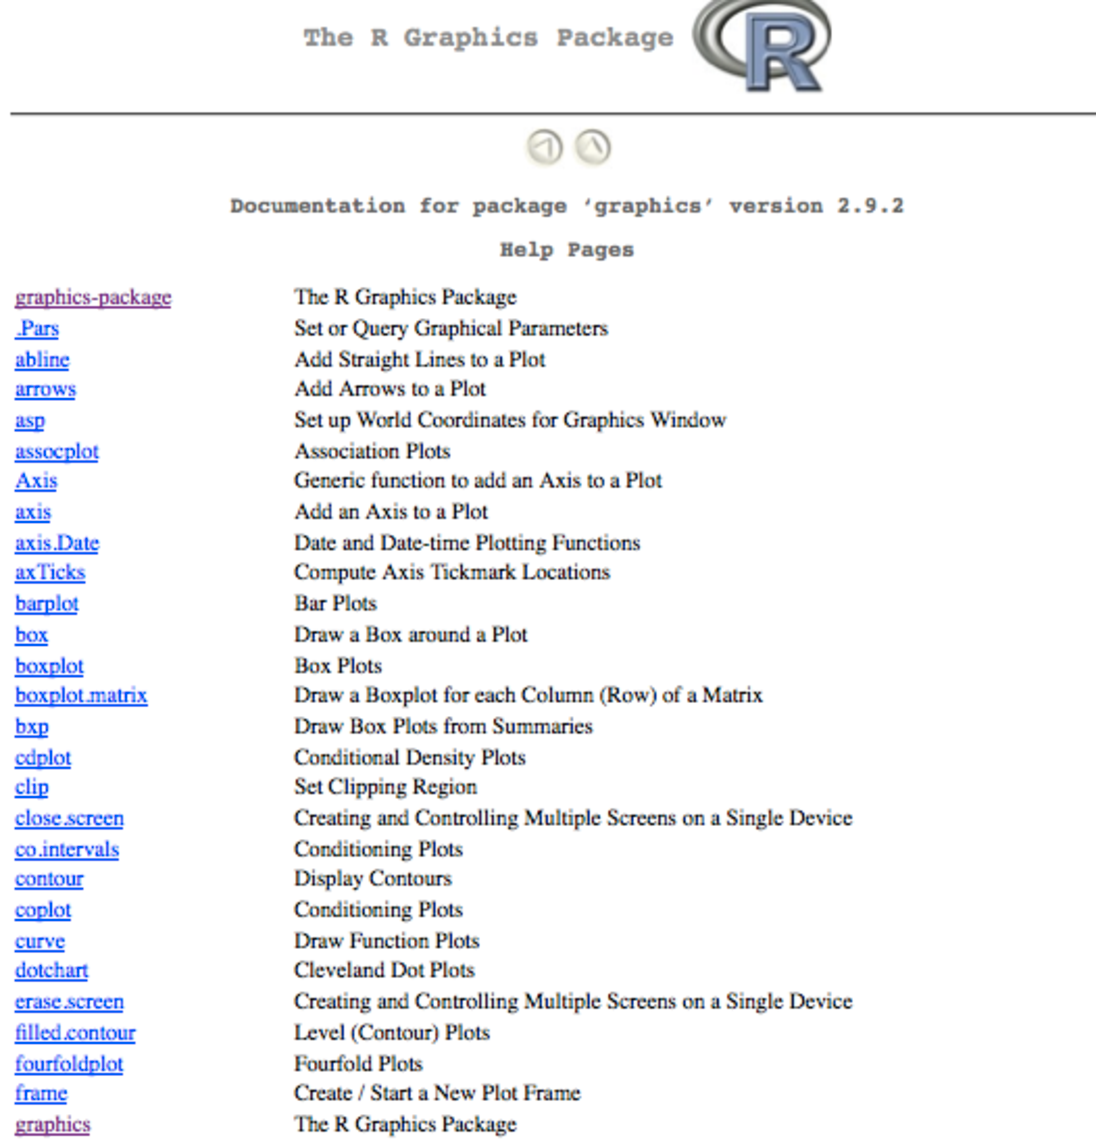
\includegraphics[height=0.65\textheight]{helpscreenshot.pdf}
\end{figure}

\end{frame}  

\begin{frame}[fragile,squeeze]{Functions}{Reading the documentation}
  \begin{columns}[t]
    \column{0.4\textwidth}
    \textbf{Commands}
    \begin{itemize}
      \item<1> \ri{help()} (\ri{?}) \only<1>{ - Function documentation }
      \item<2> \ri{help(package=\emph{package name})} \only<2> { - Package documentation listing}
      \item<3> \ri{help.search()} (\ri{??})  \only<3> { - Search \emph{all} documentation for occurances of the given term.}
      \item<4> \ri{help.start()}  \only<4> { - Open \emph{HTML} help browser in the default web browser.}
      \item<5> \ri{example()}  \only<5> { - Execute any example code in a function's documentation.  These examples should \emph{never} fail. }
      \item<6> \ri{function name} (without parenthesis)  \only<6> { - Show function body. }
    \end{itemize}
    \column{0.6\textwidth}



\begin{onlyenv}<1>\begin{minipage}{\textwidth}
\begin{Schunk}
\begin{Sinput}
>help(ls);
>?ls
>?`+`  # use backquotes when R doesn't
\end{Sinput}
\end{Schunk}
\end{minipage}\end{onlyenv}

\begin{onlyenv}<2>\begin{minipage}{\textwidth}
\begin{Schunk}
\begin{Sinput}
># help(package=RInterval); 
># truncated for space
>cat(paste(help(package=RInterval)$info[[1]], collapse="\n"), '\n');
\end{Sinput}
\begin{Soutput}
Package:       RInterval
Type:          Package
Title:         Package for efficiently dealing with
               genomic intervals
Version:       0.14
Date:          2009-09-09
Author:        David M. Rosenberg
Maintainer:    Who to complain to
               <rosenbergdm@uchicago.edu>
Description:   Classes and methods for efficiently
               analyzing single dimension genomic
               intervals, with an emphasis on copy
               number variation.
License:       LGPL
LazyLoad:      yes
Packaged:      2009-09-10 17:19:11 UTC; root
Built:         R 2.9.2; ; 2009-10-15 17:33:27 UTC;
               unix 
\end{Soutput}
\end{Schunk}
\end{minipage}\end{onlyenv}


\begin{onlyenv}<3>\begin{minipage}{\textwidth}
\begin{Schunk}
\begin{Sinput}
>help.search('digest');
\end{Sinput}
\end{Schunk}
\end{minipage}\end{onlyenv}


\begin{onlyenv}<4>\begin{minipage}{\textwidth}
\end{minipage}\end{onlyenv}

    
\begin{onlyenv}<5>\begin{minipage}{\textwidth}
\begin{Schunk}
\begin{Sinput}
>example(is.integer);
\end{Sinput}
\begin{Soutput}
is.ntg>  ## as.integer() truncates:
is.ntg>  x <- pi * c(-1:1,10)

is.ntg>  as.integer(x)
[1] -3  0  3 31
\end{Soutput}
\end{Schunk}
\end{minipage}\end{onlyenv}


\begin{onlyenv}<6>\begin{minipage}{\textwidth}
\begin{Schunk}
\begin{Sinput}
>isTRUE;
\end{Sinput}
\begin{Soutput}
function (x) 
identical(TRUE, x)
<environment: namespace:base>
\end{Soutput}
\begin{Sinput}
>lsf.str;
\end{Sinput}
\begin{Soutput}
function (pos = -1, envir, ...) 
{
    if (missing(envir)) 
        envir <- as.environment(pos)
    ls.str(pos = pos, envir = envir, mode = "function", ...)
}
<environment: namespace:utils>
\end{Soutput}
\end{Schunk}
\end{minipage}\end{onlyenv}


\end{columns}
\end{frame}

% subsection what_does_that_do_ (end)


\section{Style}

\subsection{Submissions}

\begin{frame}[fragile]{Style}{Submissions}

\begin{block}<+->{Example and template}
  An example and a template for how I'd like you to \emph{try} to submit your homework to me will be available by tonight.
\end{block}

The ``submission'' style guidelines are primarily to speed my grading of homework.

\begin{itemize}
  \item Each assignment should be submitted as a \emph{single} \cc{.R} file.  Additional (non-\cc{.R}) files / hard copies may be necessary, including
  \begin{itemize}
    \item Plots
    \item Analytical problems
    \item Data tables
  \end{itemize}
  
  \item Anything in the assignment which is not \R code should be commented out (preceded by pound signs).
  \end{itemize}
  
\end{frame}  
  
\begin{frame}[fragile]{Style}{Submissions}
  \begin{block}<1>{File header}
    The following header should start your \cc{.R} file (the first three lines may be omitted).  Substitute the relevant information for each all-caps slot.
  \end{block}

{\scriptsize\begin{semiverbatim}
\invisible<2->{#!/usr/bin/env r
# encoding: utf-8
# 
# name: STUDENT_NAME
# assignment: ASSIGNMENT_NUMBER
# date: DATE_OF_SUBMISSION
# filename: NAME_OF_FILE}
\end{semiverbatim}}


%\end{frame}  
  
%\begin{frame}[fragile]{Style}{Submissions}

 \begin{block}<2>{Question header}
    The following block should be inserted before each answer.
  \end{block}


{\scriptsize\begin{semiverbatim}
\uncover<2->{#/--#########################################################################}
\uncover<2->{# name: STUDENT_NAME}
\uncover<2->{# assignment: ASSIGNMENT_NUMBER}
\uncover<2->{# date: DATE_OF_SUBMISSION}
\uncover<2->{# question: QUESTION_NUMBER}
\uncover<2->{# subquestion: SUBQUESTION_LETTER_IF_PRESENT_OTHERWISE_EMPTY}
\uncover<2->{# other files: NAMES_OF_OTHER_RELATED_FILES}
\uncover<2->{##########################################################################/--}
\end{semiverbatim}}

\end{frame}


\subsection{Rules}


\begin{frame}[fragile,squeeze]{Style}{Rules}
      \begin{tabular}{cp{8cm}}
        \toprule
        Category & Description \\
        \midrule
        variable names & Variable names should describe their function and follow a consistent capitalization scheme \\
        indentation & \emph{code blocks} (generally delimited by brackets) should be indented (recommended 2 spaces) relative to surrounding code \\
        blank lines & use blank lines to separate independent ``chunks'' or concepts \\
        spaces & blank spaces should surround symbols and parentheses \\
        comments & comments should be used liberally to explain code and concepts \\
        line length & Individual lines should be no more than 80 characters long.  Continuation lines (if necessary) should be indented relative to surrounding code \\
        \bottomrule
      \end{tabular}
\end{frame}


\subsection{The golden rule}


\begin{frame}{Style}{The golden rule}
  
  \begin{alertblock}{The Golden Rule}
  Whatever your personal stylistic preferences / conventions are, \textbf{be consistent}.
\end{alertblock}
  
\end{frame}

%\begin{frame}[<+->] 
%  \begin{theorem}
%    $A = B$. 
%  \end{theorem}
%  \begin{proof}
%    \begin{itemize}
%      \item Clearly, $A = C$. 
%      \item As shown earlier, $C = B$. 
%      \item<3-> Thus $A = B$. 
%    \end{itemize}
%  \end{proof}
%\end{frame}

% 
% \begin{frame}{Make Titles Informative.}
% 
%   You can create overlays\dots
%   \begin{itemize}
%   \item using the \texttt{pause} command:
%     \begin{itemize}
%     \item
%       First item.
%       \pause
%     \item    
%       Second item.
%     \end{itemize}
%   \item
%     using overlay specifications:
%     \begin{itemize}
%     \item<3->
%       First item.
%     \item<4->
%       Second item.
%     \end{itemize}
%   \item
%     using the general \texttt{uncover} command:
%     \begin{itemize}
%       \uncover<5->{\item
%         First item.}
%       \uncover<6->{\item
%         Second item.}
%     \end{itemize}
%   \end{itemize}
% \end{frame}
% 
% 
% \subsection{Second Subsection}
% 
% \begin{frame}{Make Titles Informative.}
% \end{frame}
% 
% \begin{frame}{Make Titles Informative.}
% \end{frame}
% 
% 
% 
% \section*{Summary}
% 
% \begin{frame}{Summary}
% 
%   % Keep the summary *very short*.
%   \begin{itemize}
%   \item
%     The \alert{first main message} of your talk in one or two lines.
%   \item
%     The \alert{second main message} of your talk in one or two lines.
%   \item
%     Perhaps a \alert{third message}, but not more than that.
%   \end{itemize}
%   
%   % The following outlook is optional.
%   \vskip0pt plus.5fill
%   \begin{itemize}
%   \item
%     Outlook
%     \begin{itemize}
%     \item
%       Something you haven't solved.
%     \item
%       Something else you haven't solved.
%     \end{itemize}
%   \end{itemize}
% \end{frame}


\end{document}


